\chapter{Metamaterial Microwave Absorber (MMA) and its Cryogenic Applications}
\label{ch:mma}
The following was published in Applied Optics in 2020~\cite{Xu_2021}.  The paper was selected as Editor's Pick and given a press release here~\cite{MMApress}.
\section{Introduction}
Modern ground-based millimeter-wave telescope receivers have advanced to the point where detector noise is dominated by photon noise, meaning the thermal or electronic noise intrinsic to the detectors (and the associated readout system) is less than the photon noise from the incident light. The in-band optical power incident on the detectors---closely related to the photon noise---arises from the sky signal, the atmosphere, and stray light outside the desired optical path. The out-of-band instrument spectral and angle response is largely set by filter stack and baffle implementation.

The sky signal and the atmosphere power loading observed by the detectors cannot be reduced by improving the instrument, whereas the stray light loading can be reduced by a more effective design. Instead of following the main optical path, stray light is reflected or scattered by the side walls of cryogenic receivers before being absorbed by the detectors. Therefore, stray light can not only compromise image fidelity through ghosting or glint, but also degrades the detector sensitivity. In this paper, we concentrate on suppressing stray light by minimizing reflection and scattering within cryogenic receivers~\cite{iuliano/etal:2018, thornton/etal:2016, sharp/etal:2008}.

Terminating stray light at the lowest possible temperature is typically achieved by cryogenic baffling design, which minimizes reflection and scattering.  Ideally, the baffling surfaces are constructed of millimeter-wave absorbing material, with high absorptivity and low reflection/scattering over a wide range of incident angles and frequencies. Beyond the required optical properties, the absorbers should be efficiently cooled to cryogenic temperatures with robust thermal contacts and be able to withstand the mechanical stress associated with thermal cycling. Since cryogenic space is scarce, the absorbing material is often required to be as compact as possible. Ideally, the absorber should be light in mass, especially for future space missions.

Available options include conductively-loaded-epoxy~\citep{Wollack2008}, and commercially-available absorptive sheets\footnote{For example, HR-10 sheets from Emerson\,\&\,Cummings.}/tiles\footnote{For example, Tessellating Terahertz Radar Absorbing Materials (RAM), Thomas Keating Ltd.}. The conductively-loaded-epoxy relies on the conductive materials to absorb the radiation; however, the high index of refraction of the epoxy gives high reflectance and scattering, depending on the roughness of the surface. In addition, the epoxy normally has a $>$\,2\,g$\cdot$cm$^3$ density, adding a significant mass to the cryogenic system. The commercially-available absorptive sheets and tiles provide high absorption, while mechanically and cryogenically attaching them to low-temperature surfaces poses great challenges. Recent development on 3D printing also enables more absorber designs~\cite{petroff/etal:2019}, while mass production at low cost is still a challenge. To overcome these obstacles, we developed injection-molded tiles with a metamaterial gradient index anti-reflection coating. Metamaterials are artificially engineered materials, in terms of content and geometry, to achieve physical properties that are not available in nature~\cite{wollack/etal:2016, ding/etal:2012, watts/liu/padilla:2012}. Our solution provides high absorption with customized thermal and mechanical interface for cryogenic applications. 

We describe the design (Section~\ref{sec:optical_design}) and characterization (Section~\ref{sec:optical_testing}) of the tiles, along with its application within the Simons Observatory (SO) Large Aperture Telescope Receiver (LATR)~\cite{zhu18, orlo18} and Small Aperture Telescopes (SAT)~\cite{ali20}.\footnote{The MMA tiles are also used in CCAT-Prime cam~\cite{vavgiakis/etal:2018}.} We also discuss potential future applications in Section~\ref{sec:future_applications}.
\begin{figure}[H]
    \centering
    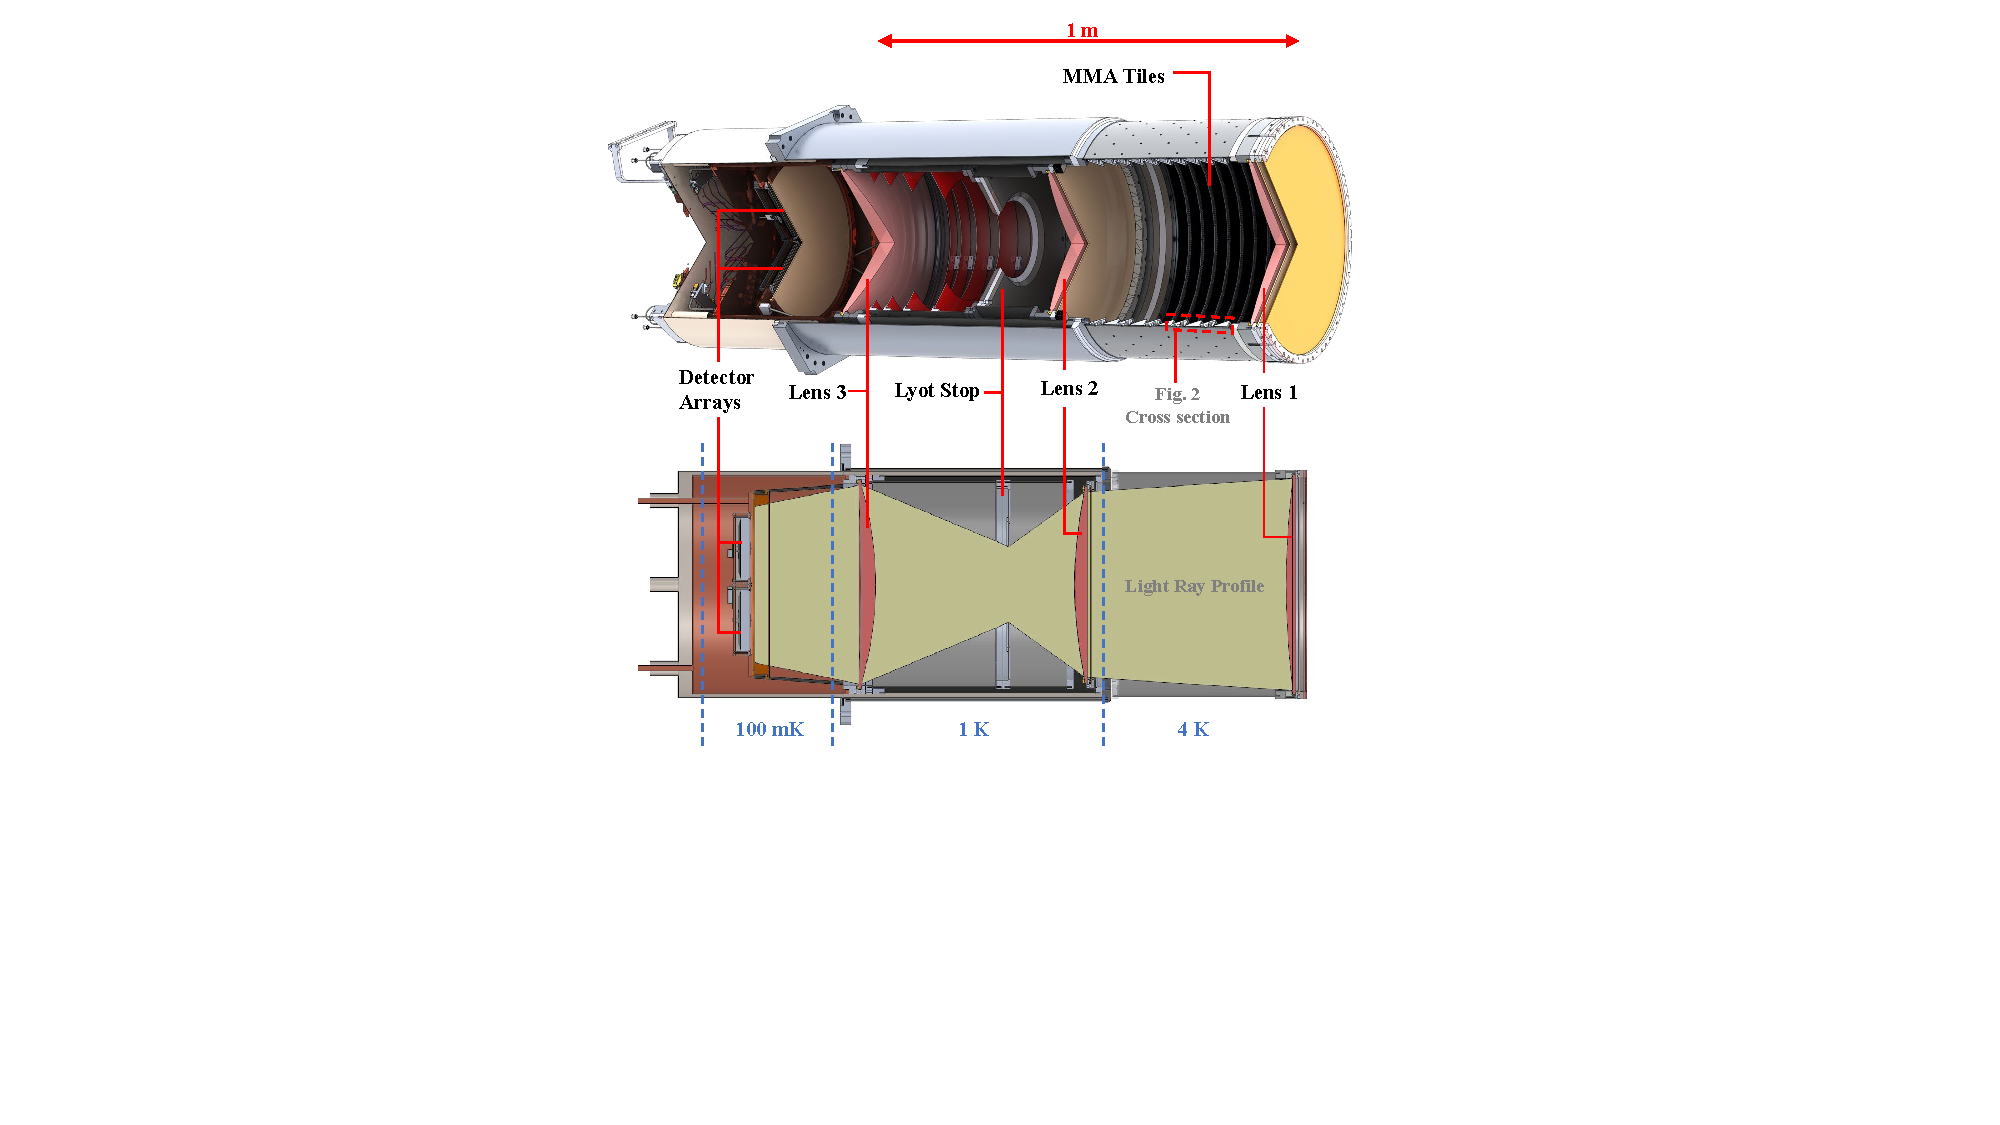
\includegraphics[width = .7\textwidth]{Figures/latr_ot.pdf}
    \caption{Large Aperture Telescope Receiver (LATR) optics tube in the Simons Observatory. A detailed rendering of the optics tube design is shown in the upper part, and a simplified schematic cross-section is shown in the bottom part. Incoming light enters the optics tube from the right and focuses on the detector arrays on the left via three lenses. The yellow-shaded region in the bottom part shows the geometric light ray profile. Operational temperatures for different parts of the optics tube are also annotated. More details of the optics tubes are described in~\cite{xu/etal:2020c}. The MMA tiles are installed in the regions between lens\,1 and lens\,2 at 4\,K. Fig.~\ref{fig:tile_design} shows a cross-section of the MMA tile assembly (box with red dashed lines) in the optics tube and the detailed design of one tile. A flat version of the MMA tile (Section~\ref{sec:future_applications}) was also used to cover the front and back of the Lyot stop at 1\,K.}
    \label{fig:latr_ot}
\end{figure}

\section{Optical Design}
\label{sec:optical_design}

The ideal baffling material minimizes reflection and scattering of light over the relevant range of angles of incidence, while mechanically (and even cryogenically) fitting within optical systems.  In the case of the SO LATR~\cite{xu/etal:2020c, zhu18, orlo18, coppi/etal:2018}, the desire to close-pack the optics tubes limits the radial extent of the absorbing material to about 1\,cm to avoid clipping the beam near the front of the optics tubes (between Lens\,1 and Lens\,2 in Fig.~\ref{fig:latr_ot}).

\begin{figure*}
    \centering
    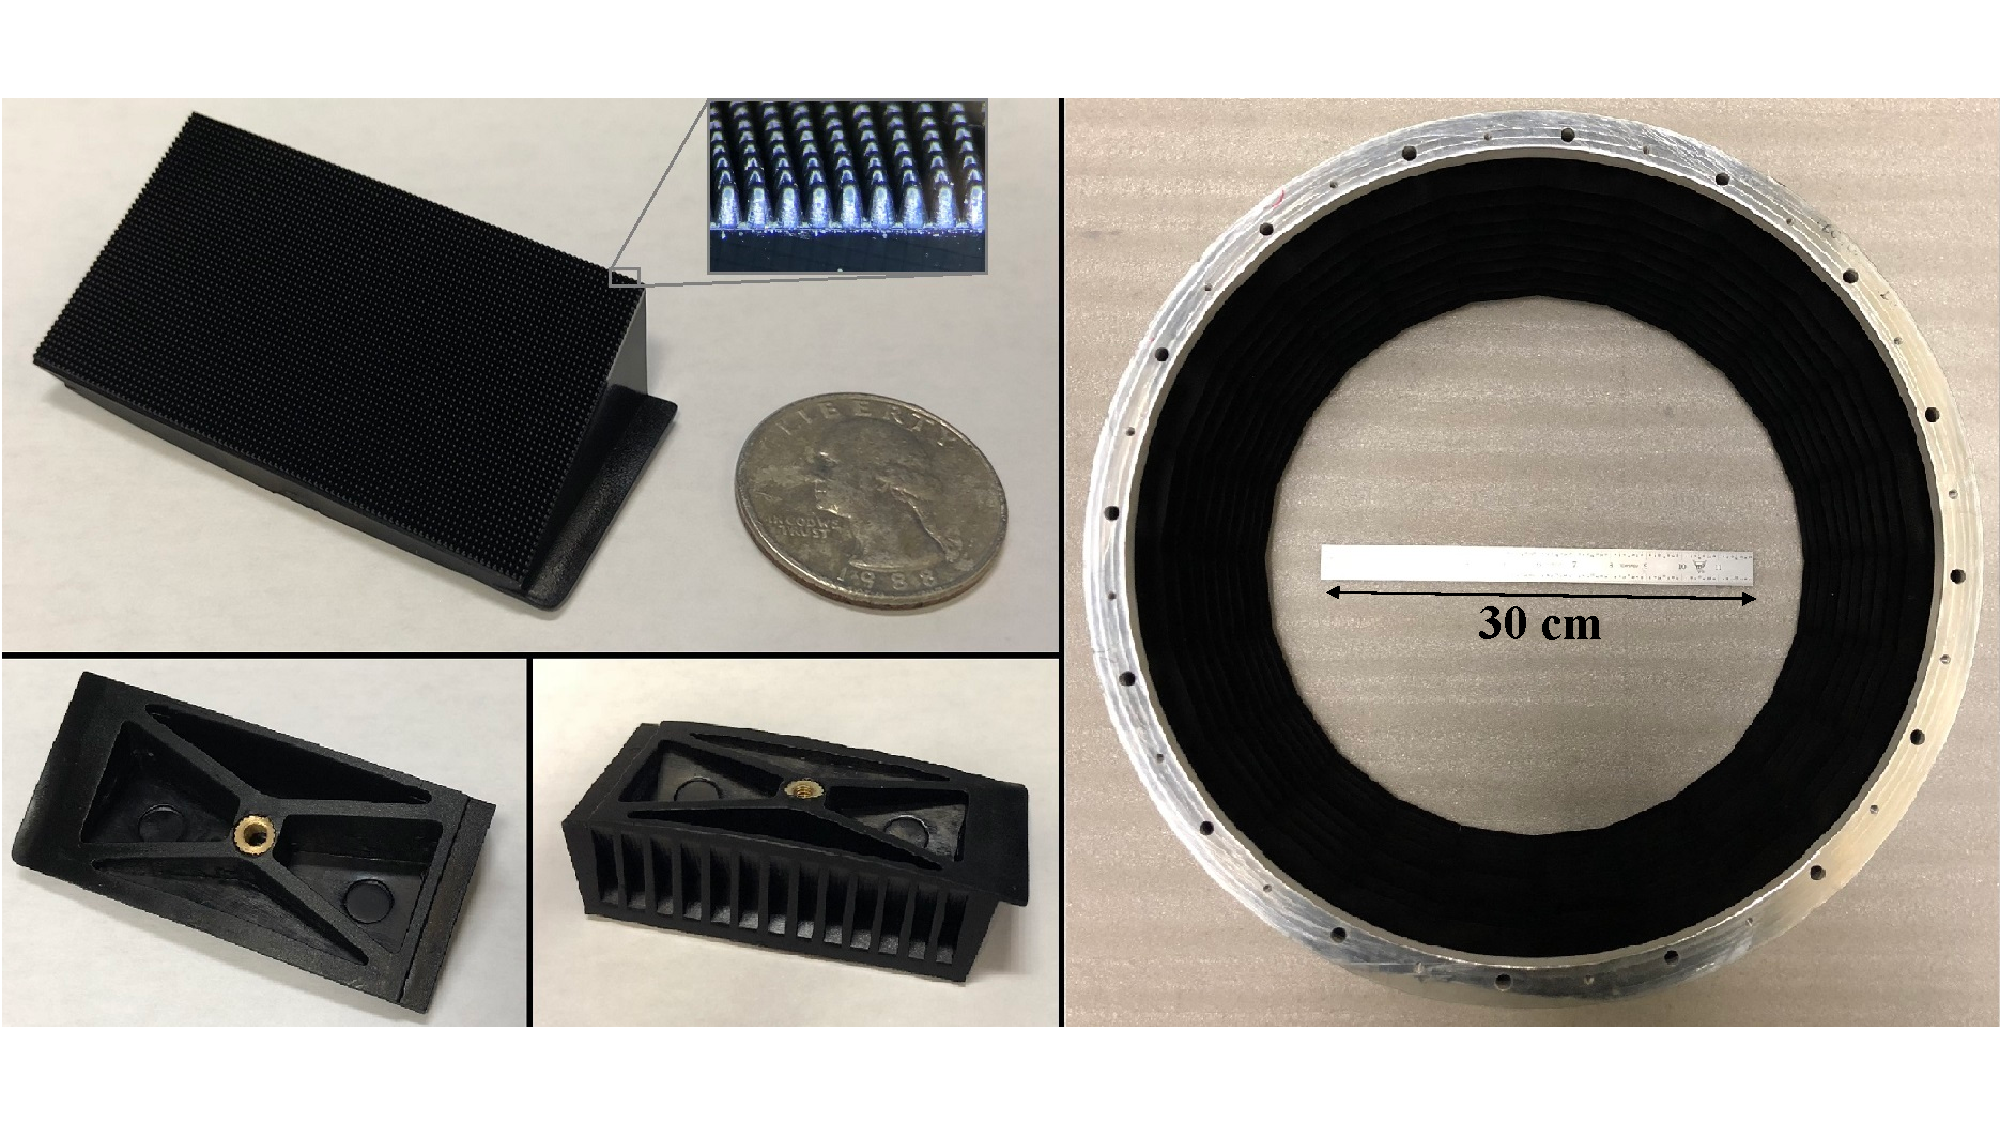
\includegraphics[width = .9\textwidth]{Figures/real_tile.pdf}
    \caption{Manufactured MMA tiles. The manufactured tiles are presented from different perspectives. The top left photo shows one tile from the absorbing surface. A microscope photo of the pyramids is shown in the insert. The pitch between pyramids is kept as 0.6\,mm as designed. The bottom left two photos show the back of the tile from two other perspectives. The light weighting pockets are visible along with the brass injected M3 nut for fastening. The photo on the right shows the assembly of 240 tiles installed on the wall of the optics tube section (see Fig.~\ref{fig:latr_ot}). A ruler ($\sim$\,30\,cm) is placed in the center for scale. Note that the absorbing surface appears to be black and featureless in the assembly photo. The condition stays the same regardless of lighting in the room, which supports the effectiveness of the AR-coating design even in optical.}
    \label{fig:real_tile}
\end{figure*}

A detailed study of the SO LATR optics tubes revealed that improving light absorption near the front of the optics tubes would most significantly reduce optical power loading~\cite{gudmundsson/etal:2020}. This study also showed that stray light on that section of the optics tubes ranges from $55^\circ$ to $90^\circ$ relative to the surface normal, taking up $\sim$\,2\,\% of the solid angle. Controlling the stray light in that section improves the telescope's mapping speed by 40\,--\,80\%,\footnote{Mapping speed is defined as $1/\textrm{NET}^2$, where NET is the noise-equivalent-temperature (NET). More details about mapping speed are available in \cite{hill/etal:2018}.} significantly increasing the sensitivity of the instrument. The Fresnel Equations show that the reflectance for dielectric materials approaches unity near grazing angles.  To improve performance at these high angles the absorbers were fabricated with the absorbing surface tilted at $26^\circ$ relative to the normal of the optics tube surface (Fig.~\ref{fig:tile_design}). The tilting reduces the angle of incidence by 26\dg{} to $<64^\circ$ (incoming light cannot exceed 90\dg{} angle of incidence) where the absorbing surface provides desired optical performance. Note that the angle of incidence is viewed in a time-reverse fashion here.

The goal of mass production led to the selection of injection molding carbon-loaded plastics. The carbon content increases the optical loss of the plastic materials so that the radiation is sufficiently attenuated within a small depth of bulk materials. However, the carbon-loaded plastics have relatively high dielectric functions, leading to high reflectance on a flat surface. Therefore, an effective anti-reflection coating is designed.  The full design and thermal testing is described in~\cite{Xu_2021}.

\begin{figure*}[t]
    \centering
    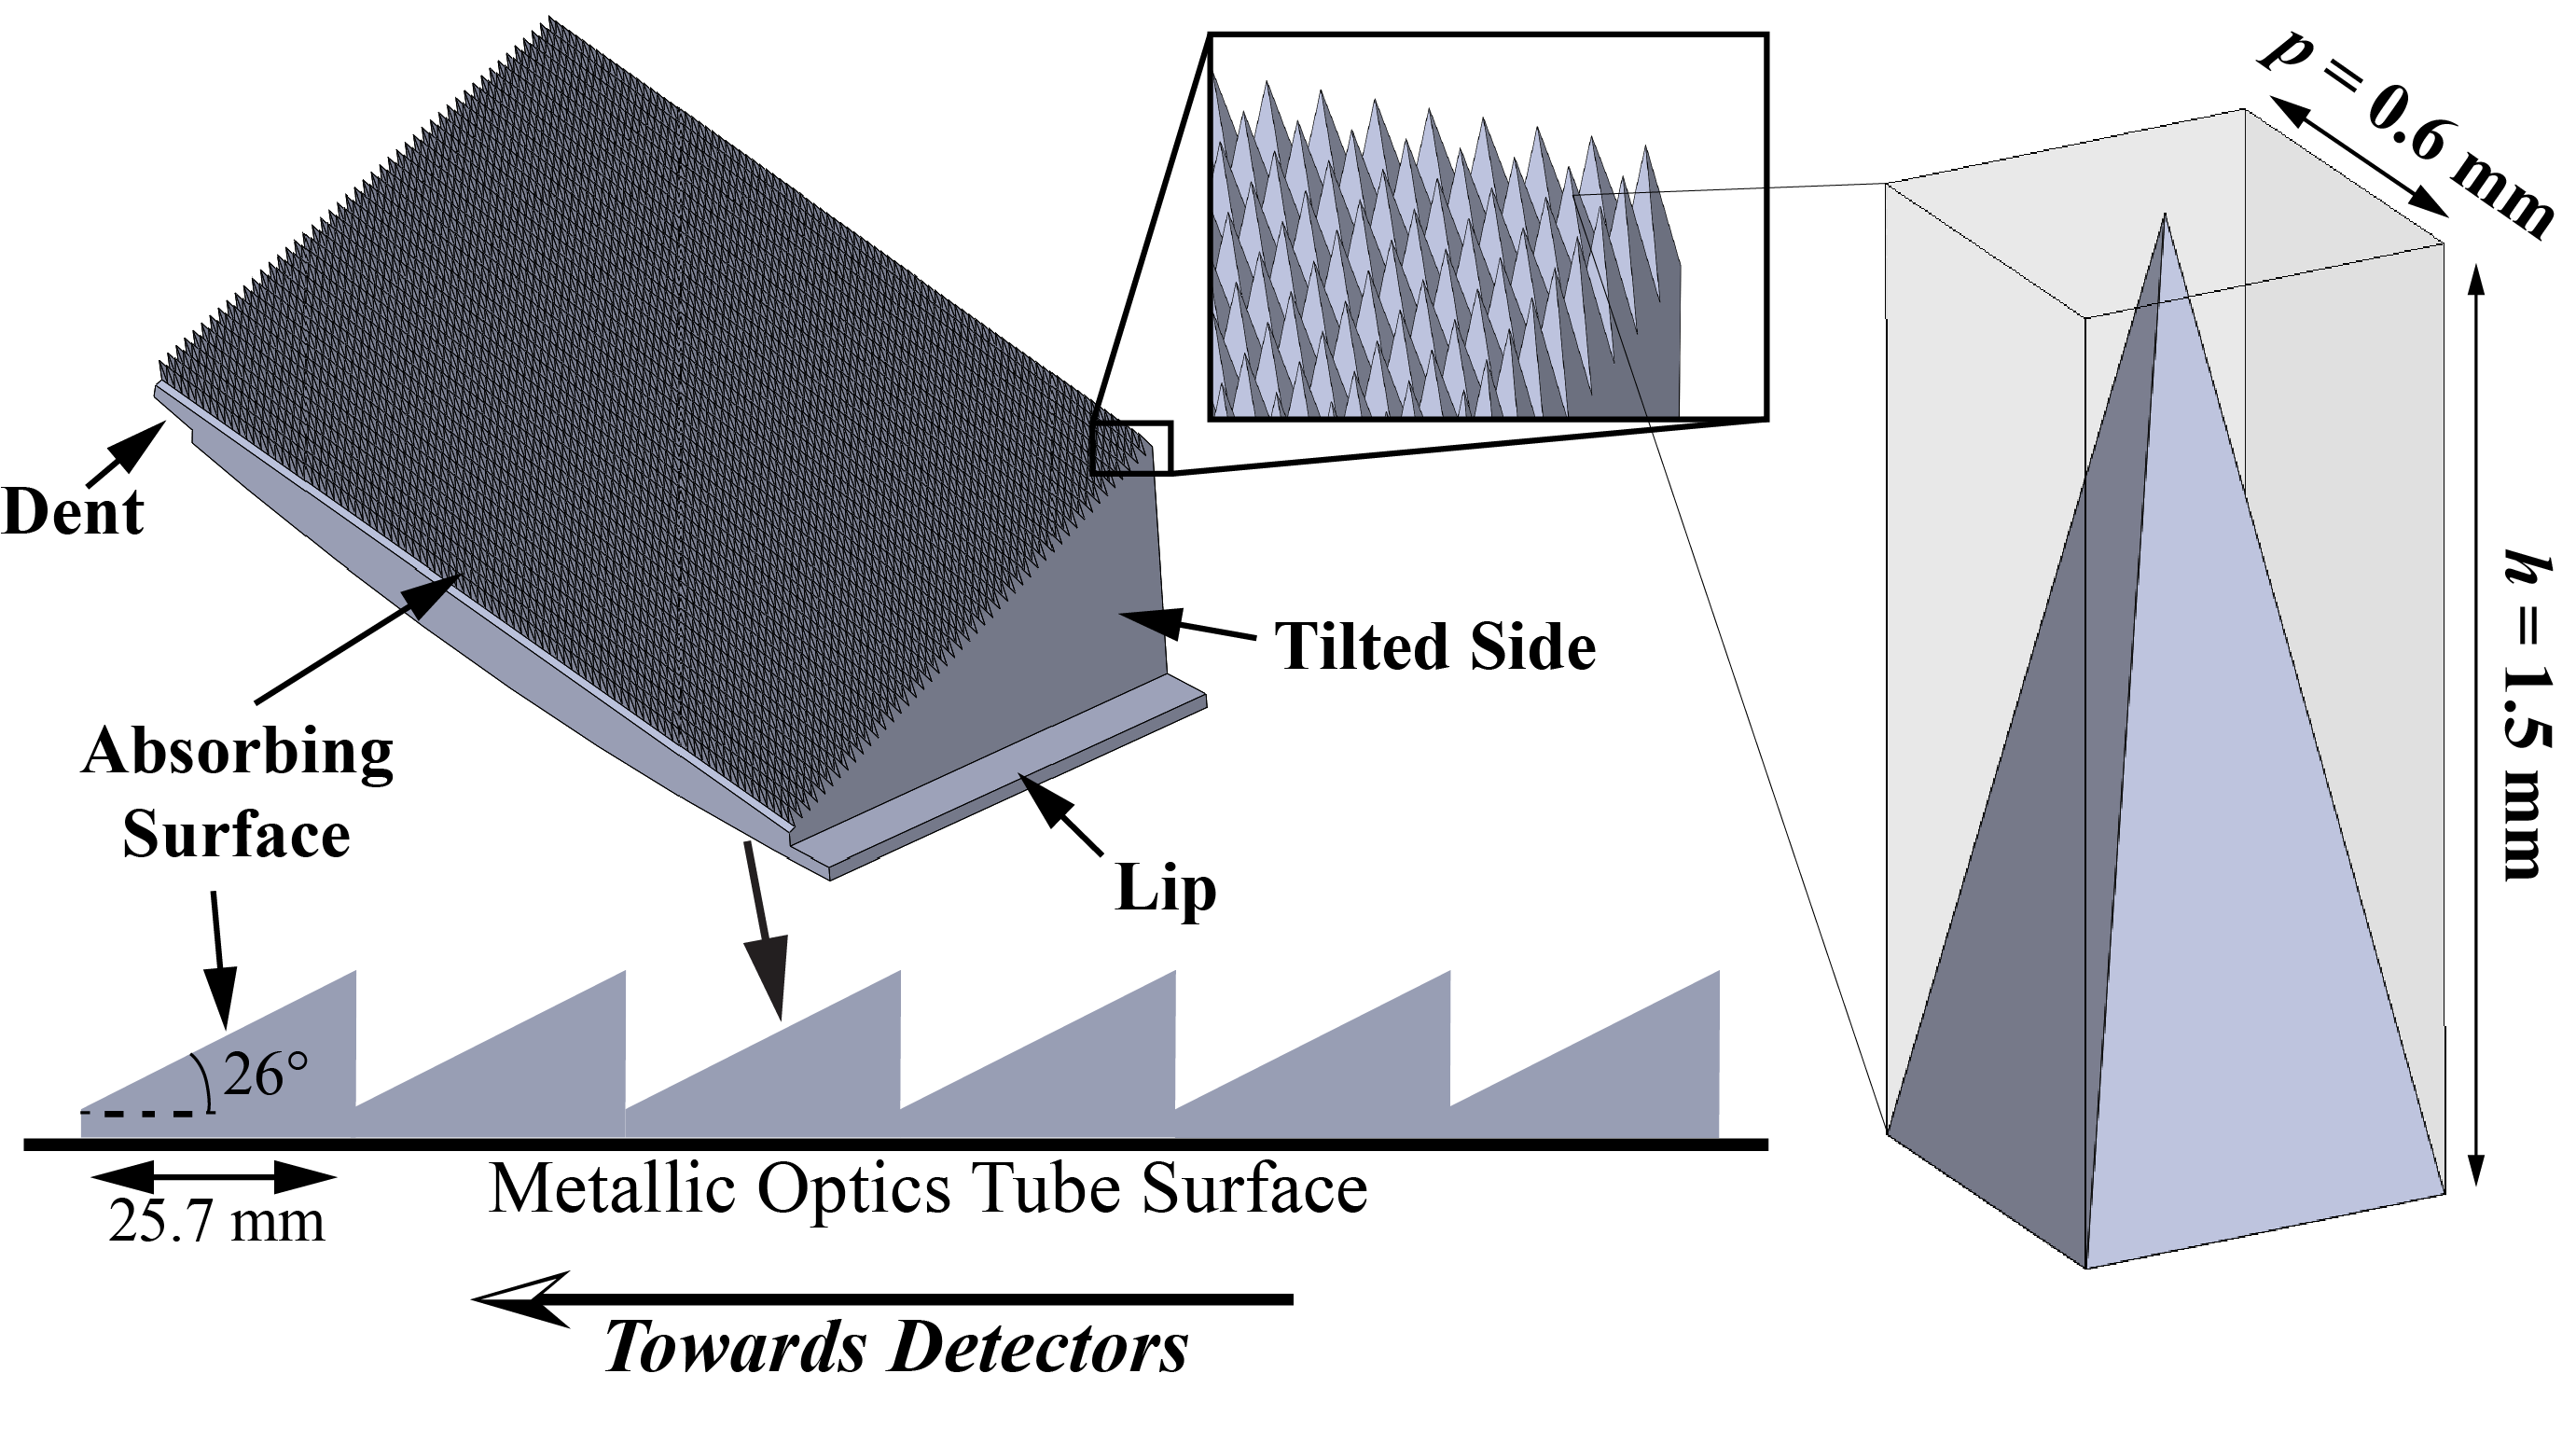
\includegraphics[width = .9\textwidth]{Figures/tile_design.png}
    \caption{MMA tile design. A snapshot of a single tile design is shown. The tilted upper surface has the pyramidal structures as described in Section~\ref{sec:optical_design}. A zoom-in plot shows details of the pyramidal structures, acting as a metamaterial anti-reflection coating. Another insert on the right zooms in further and shows one single unit of the metamaterial structure, with a pitch, $p =0.6\,$mm and a height, $h = 1.5\,$mm. The tile bottom is curved to fit the cylindrical inside surface of the metallic optics tube, which is used for structural support, heat sinking, and reflective optical termination for the absorptive tiles. A lip and a dent are for seamless tessellating. A cross-section of the segmented tilted surface is shown in the lower left part. In a time-reverse fashion, light rays coming from the left would hit the tilted surface with a <\,$64^{\circ}$ angles of incidence, where the absorbing surface achieves the desired optical performance.}
    \label{fig:tile_design}
\end{figure*}

\section{Optical Testing}
\label{sec:optical_testing}

Optical properties of the MMA tiles were measured for diffuse reflection, or scattering, at 110\,GHz and specular reflection in the frequency range from 90\,GHz to 170\,GHz. The measurements also covered different angles of incidence. The results verified that the tiles achieved the designed high absorptivity and low reflection and scattering.

The optical measurements were conducted at room temperature. A consideration in using the technology at low temperatures is the following---the detailed composition and realization of the material (e.g., amorphous lamp black, activated carbon, pyrolytic carbon, graphite, etc.) influences the temperature dependence of the bulk resistivity and thus the dielectric function of the plastic \cite{Smith1956,Sihvola2008}. From our measurement of the bulk resistivity at 3\,K relative to ambient, this is a modest effect for the carbon loaded TPU formulation explored here. The design of the MMA tiles is insensitive to the dielectric function of the bulk dielectric mixture. Therefore, dramatic changes of the tile's optical properties are not expected in cryogenic temperatures down to 3\,K or lower. 

\begin{figure*}[t]
    \centering
    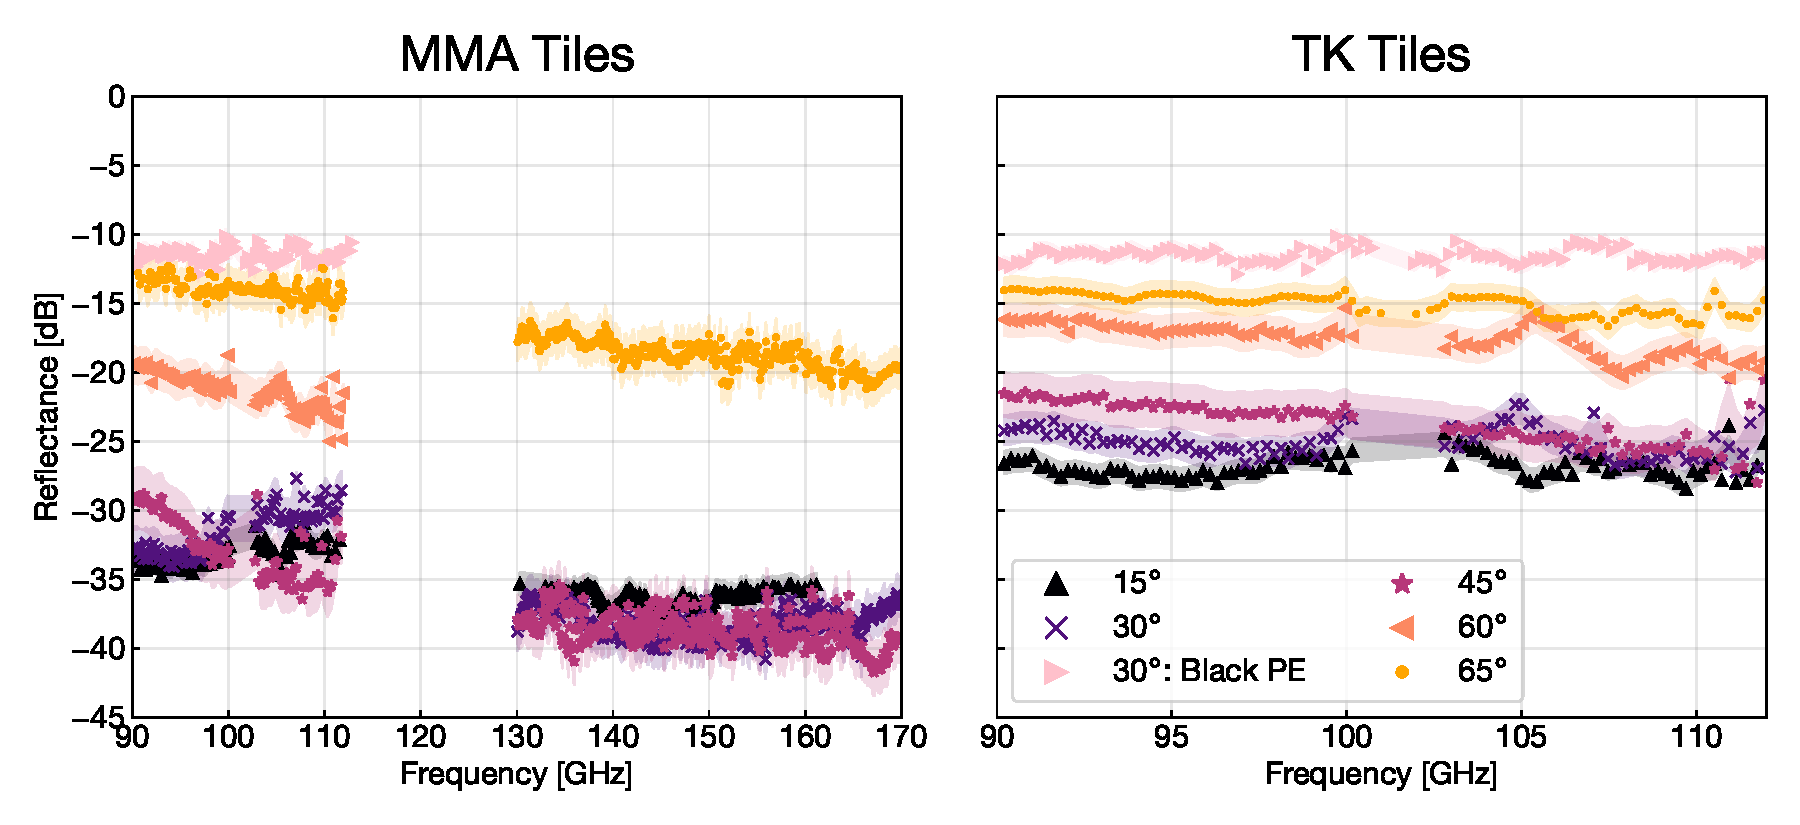
\includegraphics[width = \textwidth]{Figures/refl_2.2020.pdf}
    \caption{Specular reflectance measurements. The two panels show the specular reflectance measurements of the MMA tiles and the TK tiles at different angles of incidence, including $15^{\circ}$, $30^{\circ}$, $45^{\circ}$, $60^{\circ}$, and $65^{\circ}$. The samples are measured in W-band (90\,GHz to 110\,GHZ) and D-band (130\,GHz to 170\,GHz). The left panel shows the W-band (90\,GHz to 110\,GHZ) and D-band (130\,GHz to 170\,GHz) reflectance of the MMA tiles. The measurement gap in the left panel is due to the different frequency bands of the two sources used in the setup. The right panel measures the W-band (90\,GHz to 110\,GHZ) reflectance of the TK tiles. The two panels share the same y scale for comparison. The measurement of a flat black polyethylene sample without a AR-coating is included in both panels, which is conducted with a $30^{\circ}$ angle of incidence. Comparing the sample without an AR-coating (purple triangles) and our MMA tiles (blue crosses), $\sim$\,$-20$\,dB specular reflectance reduction is achieved with the metamaterial AR-coating.}
    \label{fig:reflection_result}
\end{figure*}


\subsection{Optical Hardware}
\begin{figure}
    \centering
    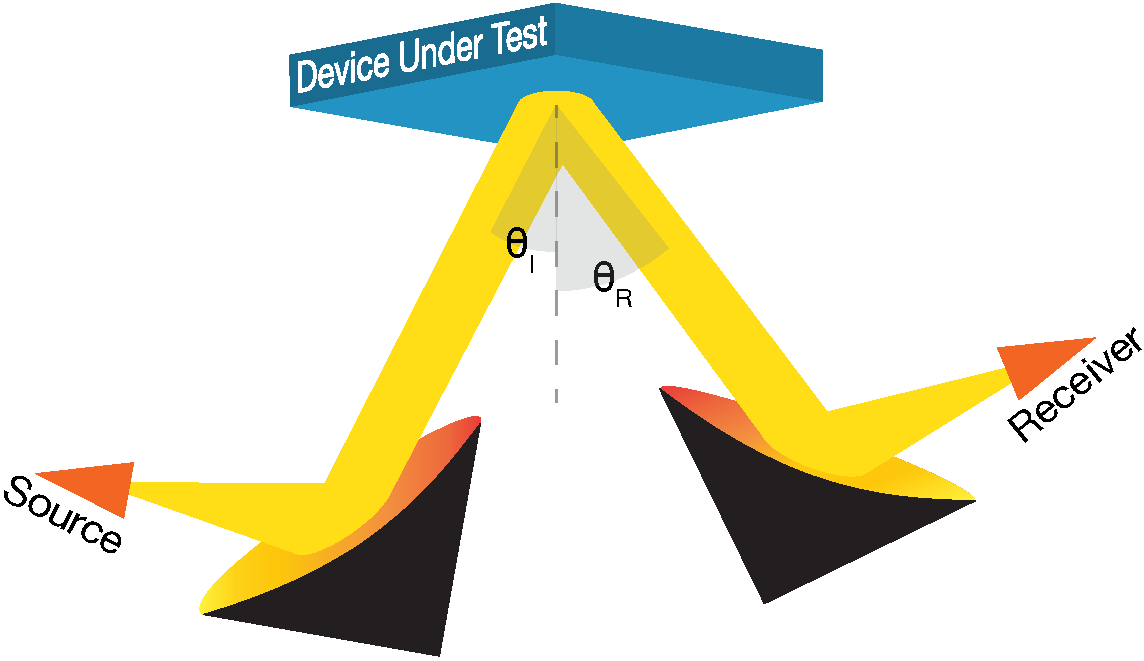
\includegraphics[width = .7\textwidth]{Figures/refl_setup.pdf}
    \caption{Optical measurement setup sketch. The orange lines represent the beam as it travels from the source feed-horn, collimated off of the first mirror and to the sample. After being reflected/scattered by the second mirror, the beam is focused into the receiver to be measured. Incident ($\theta_i$) and receiver ($\theta_r$) angles are controlled by a motor for measuring different angles of incidence and scattered power.}
    \label{fig:optical_setup}
\end{figure}
In our measurement setup, a source emits a millimeter-wave through a feed-horn toward a parabolic mirror, which then reflects a plane wave toward the sample, at an angle of incidence controlled by a rotary stage. The signal reflected off the sample propagates to a second mirror, followed by the receiver feed-horn~\cite{ches18}. The sketch of the setup is shown in Fig. \ref{fig:optical_setup}. Eccosorb HR-10 sheets are placed on surrounding surfaces to reject multipath propagation. The alignment of the receiver is controlled with a three-axis stage. The tilt of the sample is controlled with a three-point micrometer mount.

\begin{figure}[t]
    \centering
    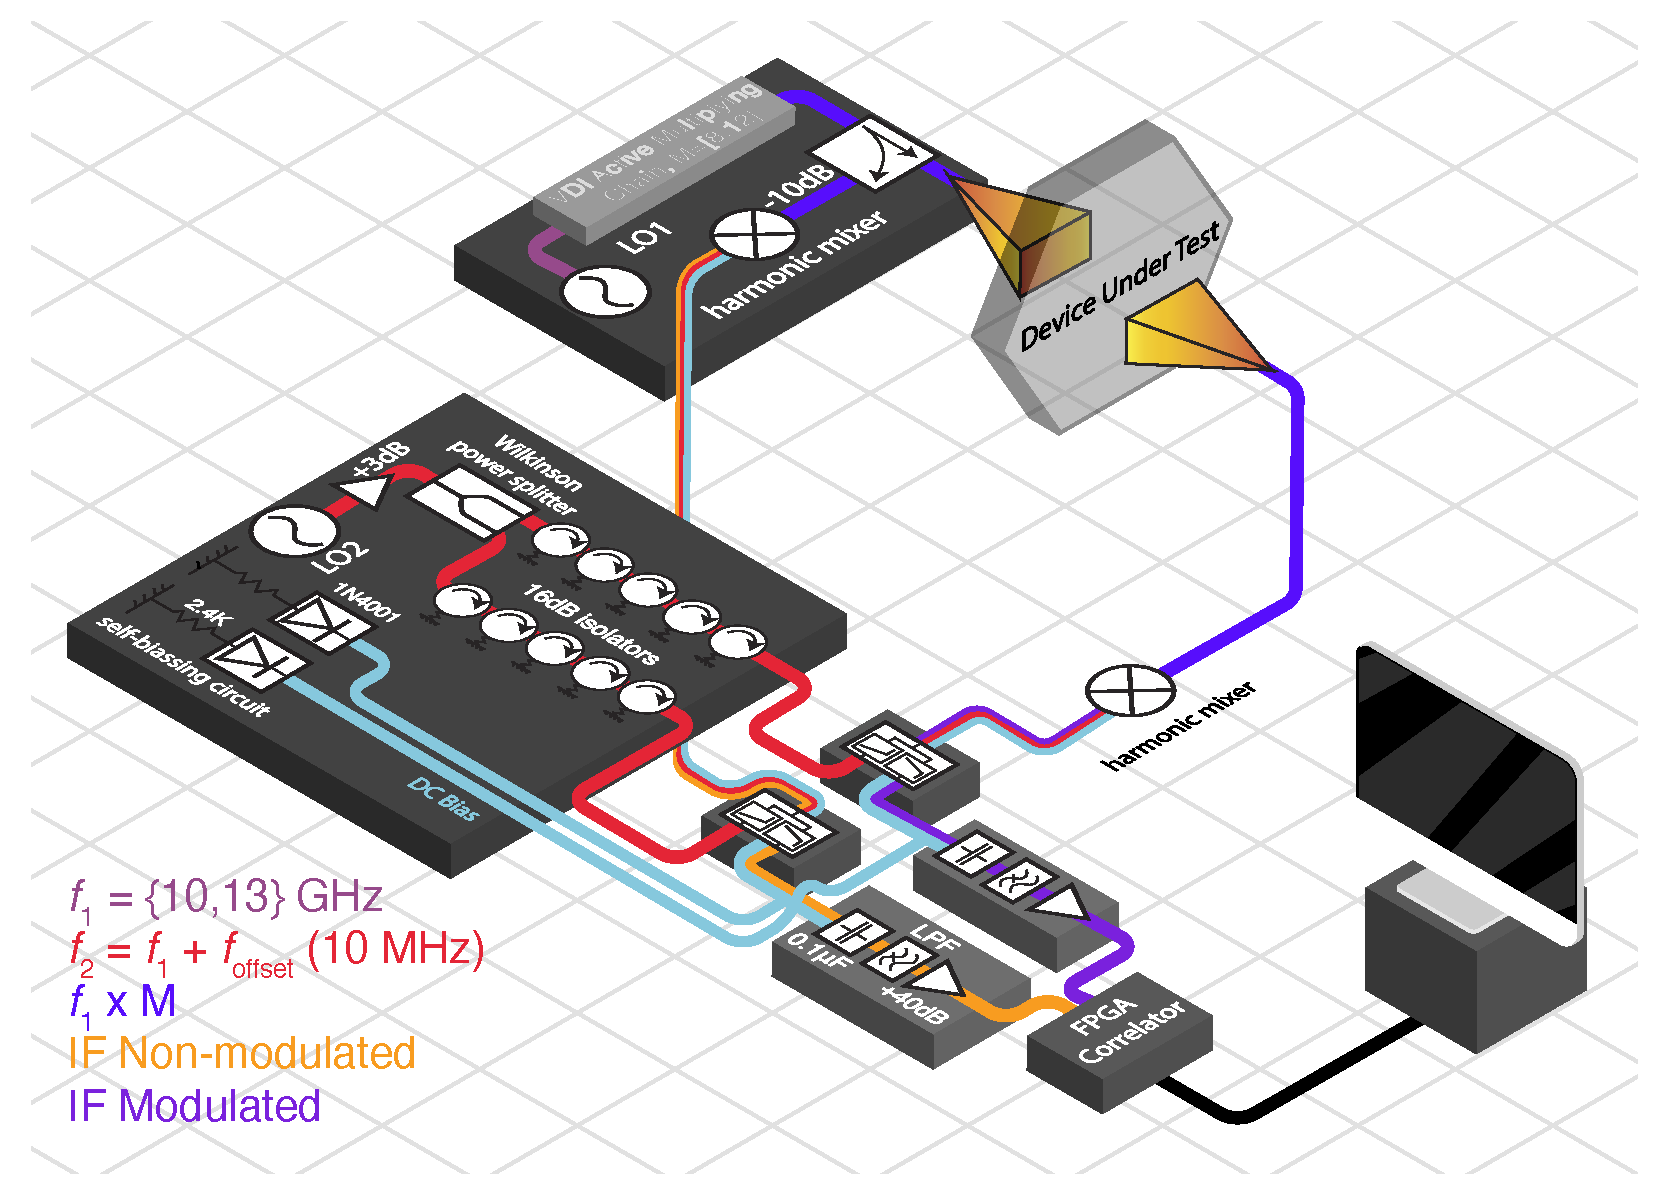
\includegraphics[width = .95\textwidth]{Figures/refl_isometric.pdf}
    \caption{The correlation receiver setup diagram. A splitter sends one signal from a millimeter-wave source to a Pacific Millimeter harmonic mixer, while sending the same signal to be modulated by the device under test. The reference and modulated signal are mixed with an LO with an offset frequency $f_{\textrm{offset}}$ from the millimeter wave source. The two Pacific Millimeter harmonic mixers extract interference information caused by $f_{\textrm{offset}}$ and sends this to the ROACH-2 field programmable gate array (FPGA) board where the two signals are correlated.}
    \label{fig:holog_ref_setup}
\end{figure}

\subsection{Receiver Electronics}

A correlation receiver is used for these measurements. The receiver compares a reference tone to a signal which has passed through the optical path, creating an interference pattern between the two~\cite{ches18}. The correlation receiver is summarized in Fig.~\ref{fig:holog_ref_setup}.  The Re-configurable Open Architecture Computing Hardware (ROACH-2) board correlates the reference and modulated signals~\cite{roach2}.

The millimeter-wave source sends a signal, ranging from 10.5\,GHz to \,13 GHz, to a multiplier which passes through a passive multiplying chain. The W-band (90\,--\,110\,GHz) and D-band (130\,--\,180\,GHz) millimeter-wave sources use multiplication factors of 9 and 12, respectively. The signal is then modulated by the sample. The modulated and the reference signals are separately sent to two harmonic mixers. The mixers extract interference information caused by the offset frequency and send it to the correlation device. This receiver outputs the amplitude and phase of the signal in narrow (50 MHz) spectral bands.  Only the amplitude is used in this analysis, though we note that the phase information could be used to improve these measurements in the future.

\subsection{Measurement}

In order to measure their optical properties, an array of tiles are screwed down to a 3D-printed plate. The 3D-printed plate compensates the wedge shape of individual tiles so that absorbing surfaces of all tiles are aligned and oriented upward, forming a 30.5$\times$30.5\,cm flat surface (Fig.~\ref{fig:front_tiles}).

For comparison, we acquired the Tessellating Terahertz RAM from TK Instruments.  The TK tiles are 25\,mm $\times$ 25\,mm square tiles that can be tessellated to cover a flat surface. The pyramidal structures ($\sim$2.5\,mm in pitch and height) on the optical surface are designed to reduce the specular reflection and scattering in the 100\,--\,1000\,GHz region. 

\begin{figure}
    \centering
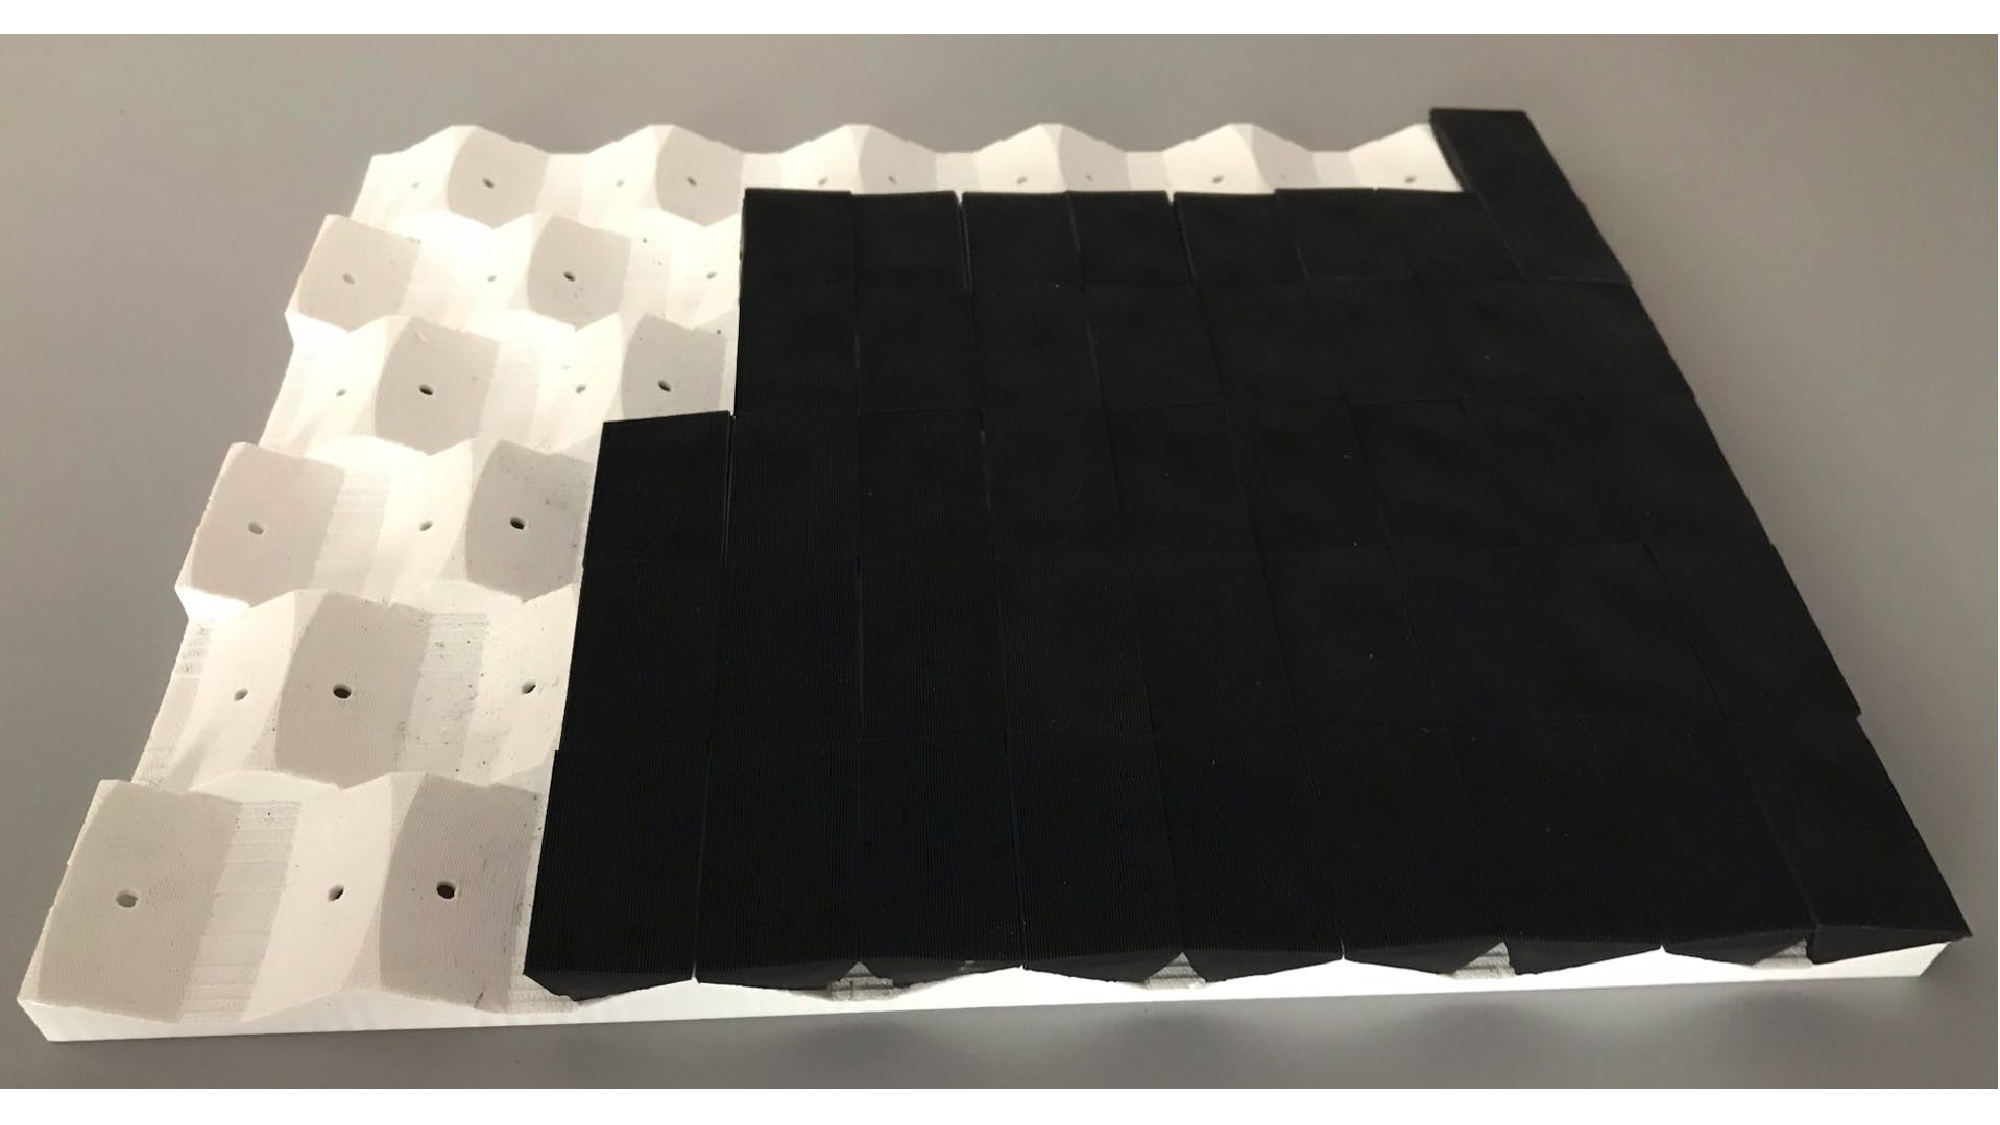
\includegraphics[width = .8\textwidth]{Figures/flat_sample.pdf}
    \caption{MMA measurement sample. MMA tiles are individually bolted into a 3D-printed plate such that each absorbing surface sits flat to form a 30.5$\times$30.5\,cm testing surface.}
    \label{fig:front_tiles}
\end{figure}

Although the TK tiles and our MMA tiles both have pyramidal structures on the optical surface, they function differently. Pyramids in our MMA tiles, with the sub-wavelength scale, act more as a layer of medium with changing index of refraction; while pyramids in the TK tiles works more within the geometric optics regime to increase the number of bounces of the incoming radiation, due to the adopted surface geometry~\cite{Chuss2017}. The TK tiles have long been the preferred absorbers in millimeter wavelengths due to their optical performance. The measurement of the TK tiles ($\geq$\,200\,GHz) are available in the product website and published literature~\cite{Saily/etal:2004}. Because our MMA tiles are optimized to perform well at our operating wavelengths, we expect an improvement in performance. Even though our measurement only verifies the performance within 90\,--\,170\,GHz, our MMA tiles are designed to work from 90\,--\,270\,GHz following the same physical principles.
\section{Reflection Measurement}

Once the setup is aligned using an aluminum plate in place of the sample, a calibration data set is taken by measuring the specular reflectance of the same aluminum plate as a function of frequency. The sample measurements are then normalized using the aluminum plate data. 

Fig.~\ref{fig:reflection_result} shows the reflected power measured for the MMA and TK samples, with the MMA tiles measured from 90\,GHz to 170\,GHz and the TK tiles measured from 90\,GHz to 110\,GHz. The measured results demonstrate the relative performance of the two. For the MMA tiles, specular reflection is at sub-percent levels (<\,-20 dB) for all angles of incidence except for $65^{\circ}$ ($\sim$\,-15\,dB). Note that $65^{\circ}$ is higher than the angle of incidence upper limit in our application (see Section~\ref{sec:optical_design}). To demonstrate the effectiveness of the anti-reflection coating, a flat carbon-loaded polyethylene (PE) sample without an AR-coating was measured. During the test, a proper flat molding material sample was not available. Therefore, we measured the carbon-black loaded PE sample---with a lower dielectric function---as a lower limit of the reflectance from a flat molding material sample. With the coating, the MMA tiles reduce the specular reflection by $\sim$\,$-20$\,dB. Meanwhile, the specular reflection from the TK tiles is 5--10\,dB higher than that from the MMA tiles at different angles of incidence.


\section{Scattering Measurement}

The scattered power off the surface of the sample is determined by measuring the received power as a function of the receiver's angle, fixing the source feed horn at a set angle (Fig. \ref{fig:optical_setup}). The source (incident) and receiver (scattered) angles are controlled by two rotary stages. The radiative source sends one frequency and is held at a constant position (i.e. angle of incidence), while the receiver sweeps across different angles. Fig.~\ref{fig:scatter} shows the scattering measurement with a 110\,GHz source at four angles of incidence: 15$^{\circ}$, 30$^{\circ}$, 45$^{\circ}$, and 60$^{\circ}$. To account for the uneven surface of the samples, scattered power is measured and averaged over 17 rotations of the sample (Fig.~\ref{fig:front_tiles}). Then error bars (in Fig.~\ref{fig:scatter}) are estimated from the 17 measurements as the standard error of the mean. The measurements show that wide-angle scattering is suppressed to <\,-40\,dB (<\,0.01\,\%). All measurements are referenced to the specular reflection data from the aluminum plate. 

\begin{figure}
    \centering
    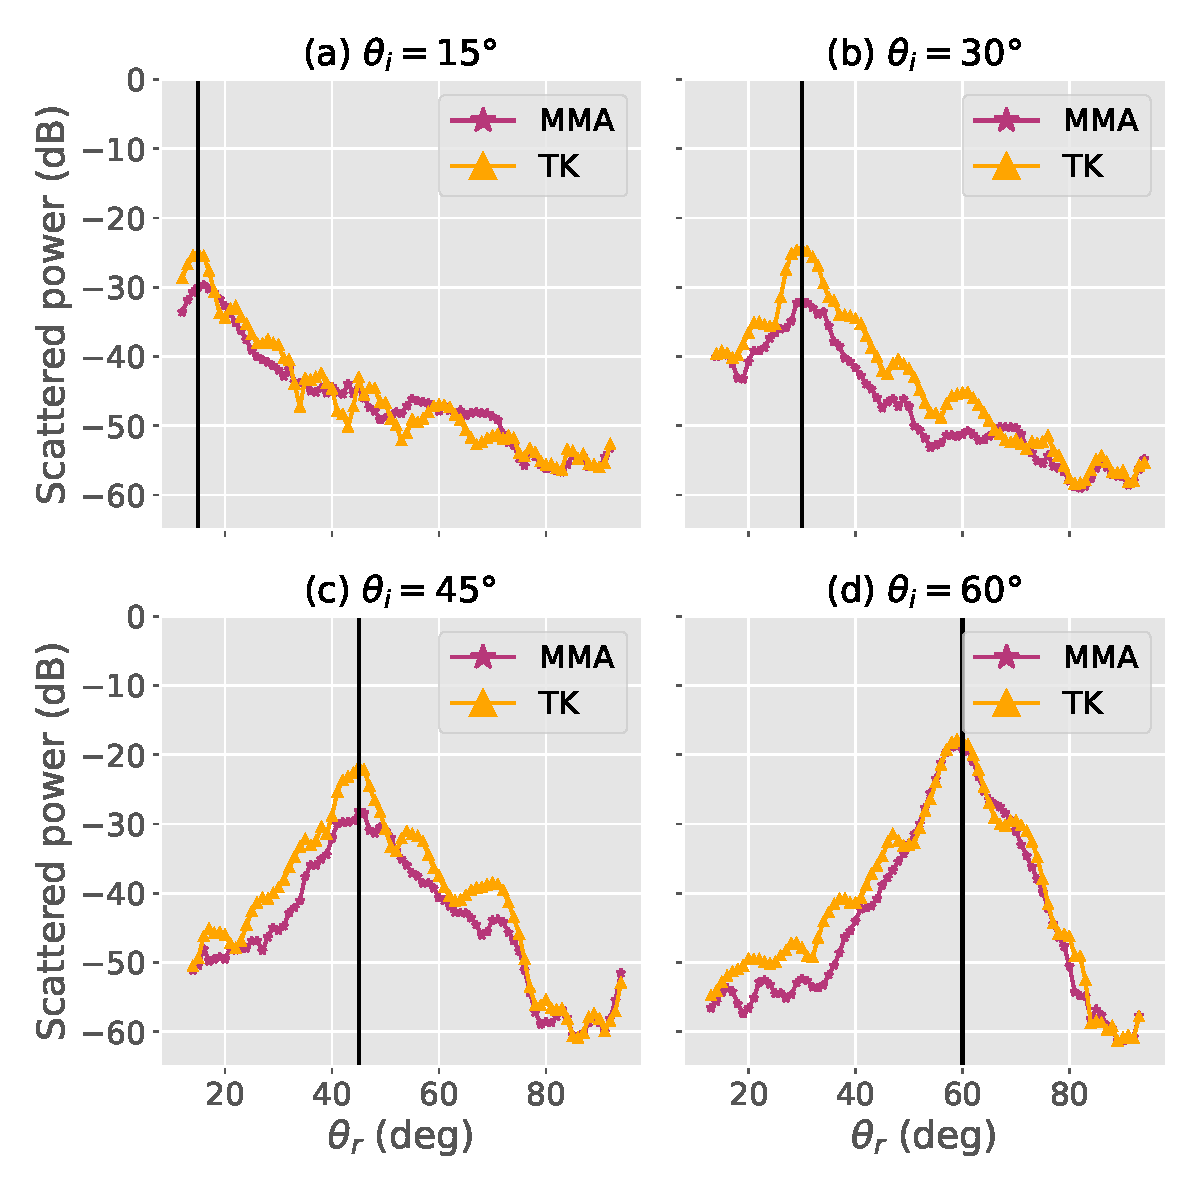
\includegraphics[width = .9\textwidth]{scatter_3_2020.pdf}
    \caption{Scattering measurement. The four panels show front scattered power off the sample with the source located at four angles of incidence $\theta_i$: (a) \,15$^{\circ}$, (b) \,30$^{\circ}$, (c) \,45$^{\circ}$, and (d) \,65$^{\circ}$. The source was set at 110\,GHz. Each of the measured data points was averaged over 17 different sample rotation angles, from which the associated error bars were also estimated. The error bars are too small to be visible at these y scales. The vertical black lines indicate the position of the specular reflection directions. The blue data points show the results from the MMA tiles, while the red data points show the results from the TK tiles. The TK tiles are measured to have an overall higher scattering than the MMA tiles, which leads to a higher integrated scattering power, as shown in Table~\ref{tab:scat}.}
    \label{fig:scatter}
\end{figure}

\begin{table}[ht]
\centering
\begin{tabularx}{0.45\textwidth}{>{\centering\arraybackslash}X >{\centering\arraybackslash}X >{\centering\arraybackslash}X}
    \hline
    \hline
    $\theta_\text{I}$ & $15^{\circ}$ & $30^{\circ}$ \\
    \hline
    MMA & $0.49\pm0.03$\% &$0.12\pm0.002$\% \\
    TK  & $0.67\pm0.02$\% &$0.53\pm0.01$\%  \\
    \hline
    \hline
    $\theta_\text{I}$ & $45^{\circ}$ & $60^{\circ}$ \\
    \hline    
    MMA & $0.27\pm0.01$\% &$1.98\pm0.02$\% \\
    TK  & $0.83\pm0.01$\% &$2.24\pm0.02$\% \\
    \hline
\end{tabularx}
\caption{Integrated scattering power (in percentage) with different source angle of incidence $\theta_\text{I}$ at 110\,GHz for MMA and TK tiles. Integration is from $\theta_\text{R}=$ $0^{\circ}$ to $45^{\circ}$ away from the specular reflection direction. The cited error is calculated from the standard error of the mean over the 17 repeated measurements for each angle of incidence.}
  \label{tab:scat}
\end{table}

The integrated scattering power is calculated by integrating the scattering over the corresponding solid angles (Eq.~\ref{eq:scat}). The sample's fractional integrated scattering power, denoted as \textit{S}, is normalized by the total integrated input power where \textit{B} is the sample measurement, \textit{A} is the normalized aluminum plate reflection and scattering profile, and $\theta_r$ is receiver angle.

\begin{equation}
\text{S} =\int_{0}^{\frac{\pi}{4}} \text{B} \sin(\theta_\text{r}) d\theta_\text{r} \bigg/ \int_{0}^{\frac{\pi}{4}} \text{A} \sin(\theta_\text{r}) d\theta_\text{r}.
\label{eq:scat}
\end{equation}

We do not include the power beyond 45\dg{} ($\pi/4$) away from the specular reflection direction, considering its negligible contribution. We calculate the integrated scattering power for our MMA tiles and the TK tiles, listed in Table~\ref{tab:scat}. The results demonstrate the MMA tiles have lower integrated scattering power compared to the TK tiles, meeting the 1\% requirement for angle of incidence $\leq 45^{\circ}$.

\section{Future Applications}
\label{sec:future_applications}
Flat and square MMA tiles were manufactured, in quantities of $> 10,000$, for more general use. The square tiles come in the size of 2.5\,cm $\times$ 2.5\,cm with the same anti-reflection coating (Fig.~\ref{fig:square_tiles}). Each of the flat tiles weigh $\sim$\,4\,g. Tessellating features cover the sides of the square tiles: two sides of the square overhang as lips, while the other two sides indent. These features enable seamlessly tessellating copious number of tiles together. Given the limited thickness ($\sim$\,6\,mm), an injected nut cannot be installed; instead a shaft was designed on the back for alignment. For fastening, four over-sized M2 screw holes were designed on the tessellating lip. Correspondingly, four recesses for the screw head (from adjacent tiles) were designed on the tessellating dent (see Fig.~\ref{fig:square_tiles}). This version of MMA tile is designed to be applied on any flat surfaces by tessellation. They are already used to cover both sides of the Lyot stop in the SO LATR optics tubes (as shown in Fig.~\ref{fig:latr_ot}). The tile-covered Lyot stop assembly has been tested at 4\,K for thermal properties. 



Given the vast potential in customization, the MMA tiles provides a viable solution to blacken cryogenic surfaces with diverse geometries. Therefore, the technology can be useful for many future cryogenic experiments.


\section{Conclusion}
\label{sec:conclusion}

The metamaterial absorber (MMA) provides an effective, novel, and low-cost solution to absorb millimeter-wave radiation at cryogenic temperatures. Once the injection mold is manufactured, the tiles are mass-produced at low cost ($<$ 1/10 of conventional methods) with a thousands-per-month production rate. Both the initial mold machining and injection molding were performed completely by an external shop, without any involvement from the research group. In addition, the technology also enables a high level of customization in the design. For future cryostat development, customized tiles can be designed and manufactured in this way to achieve the enhanced absorption properties, while fitting the geometry of specific cryostat designs.

\begin{figure}[ht]
    \centering
    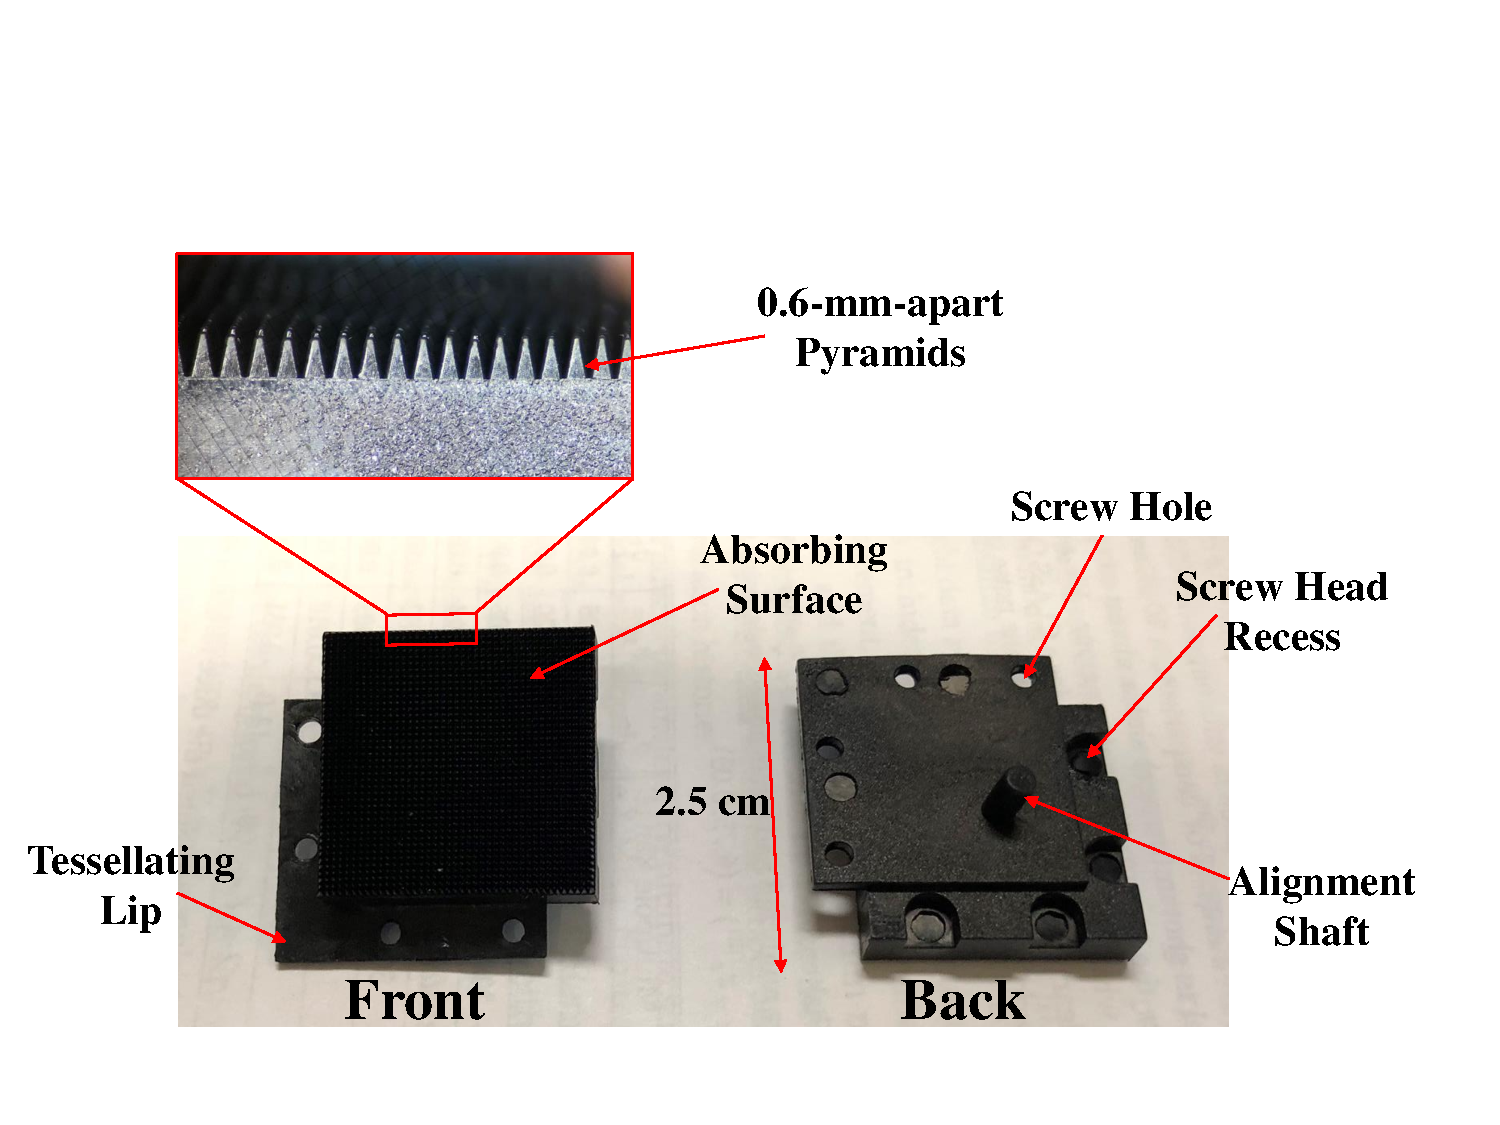
\includegraphics[width=0.8\textwidth]{Figures/square_tiles.pdf}
    \caption{Manufactured square tiles. The 2.5\,cm $\times$ 2.5\,cm flat tiles are also manufactured via injection molding with the same pyramidal structure on the absorbing surface. The main photo on the bottom shows two square tiles from the front and the back. Major features on the tiles were denoted as well. A microscope photo of the pyramids is shown on the top left. The photo shows sharp features of the pyramids, which are only 0.6-mm wide and 1.5-mm tall. The pyramids show sharper features compared to the ones in the tilted tiles (Fig.~\ref{fig:real_tile}). That is because the square tiles are smaller with a simpler shape, which facilitates the manufacturing process.}
    \label{fig:square_tiles}
\end{figure}

The absorber was successfully cooled down to 1\,K with a single thermal contact. The optical properties, including specular reflection and scattering, were measured at different angles of incidence in the frequency band from 90\,GHz to 170\,GHz. The specular reflection is $< -30$\,dB for angles of incidence $\leq45$\dg{}. Even at 65\,\dg{}, the specular reflection is only $\sim-15$\,dB. The integrated scattering power is less than 1\% with the angle of incidence $\leq45$\dg{}. Even though this application was tailored for the frequency band from 90\,GHz to 270\,GHz, the metamaterial anti-reflection coating parameters can be suitably adjusted for use at longer wavelengths. The carbon grain size of this commercially available material and the injection molding process limit the suitability of direct scaling this design to shorter wavelengths. The use of a similar dielectric mixture with carbon lamp black and a lower volume filing fraction could be employed to address this challenge.

The design philosophy breaks the overall surface into basic tiles, facilitating their application to an extended surface. Unlike painted absorbing surfaces, the modularized design allows for the easy replacement of tiles, should part of the surface be damaged. The wedge-shape tile introduced in this paper is designed to work in a specific cylinder for Simons Observatory and CCAT-Prime. But different geometries, such as flat square tiles, are also available with similar optical performance.
